\documentclass[]{article}

\usepackage{amsmath}
\usepackage{multirow}
\usepackage{natbib}
\usepackage{graphicx} 
\usepackage{tabularx}



\begin{document}

\title{Transverse-Dominant Anisotropic Dispersion and Transient Trapping in 3D Solenoidal Turbulence}

\author{Denario}
\date{Anthropic, Gemini \& OpenAI servers. Planet Earth.}

\maketitle
\begin{abstract}
The relationship between large-scale energy injection, coherent structures, and particle transport in turbulence is a fundamental problem. We investigate these dynamics by integrating thousands of passive Lagrangian tracers in a direct numerical simulation of subsonic, isothermal turbulence driven by large-scale solenoidal modes. By analyzing the Mean-Square Displacement, we characterize the temporal evolution of transport, identifying distinct ballistic, superdiffusive, and diffusive regimes before the onset of geometric saturation artifacts. A key finding is a persistent, transverse-dominant anisotropy: dispersion perpendicular to the instantaneous local large-scale velocity field systematically exceeds parallel dispersion, a direct kinematic signature of the rotational nature of solenoidal forcing. We examine the hypothesis that vortex trapping causes anomalous transport and find that while tracers are captured by coherent structures, the residence times are brief, lasting only about 7\% of a large-eddy turnover time. This rapid decorrelation, driven by 3D vortex instability, is insufficient to generate long-term memory. Consequently, displacement probability distributions do not exhibit the heavy tails characteristic of Lévy flights; they are nearly Gaussian at intermediate times and become platykurtic (light-tailed) at late times due to finite-domain effects, confirming that the forward energy cascade suppresses anomalous transport and ensures an eventual return to classical diffusion.
\end{abstract}








\section{Introduction}
\label{sec:intro}
The transport of passive tracers by a turbulent flow is a fundamental process central to phenomena ranging from pollutant dispersal in geophysical flows to star formation in the interstellar medium. A primary goal of turbulence theory is to develop predictive models for this transport by connecting the statistical properties of particle trajectories to the underlying fluid dynamics. Such models often depend on assumptions about the flow's structure, particularly regarding the mechanisms of energy injection at large scales and the role of coherent structures. The geometry of the energy input can profoundly shape the flow's topology, creating distinct pathways for particle dispersion and potentially challenging classical assumptions of isotropic, homogeneous diffusion. Understanding this connection is therefore essential for accurately modeling transport in complex, multi-scale systems.

A key distinction in turbulence is the nature of the large-scale forcing, which can be broadly categorized as either compressive (irrotational) or solenoidal (rotational). Solenoidal forcing, which conserves volume and is characteristic of many subsonic and incompressible flows, naturally generates large-scale swirling motions and long-lived coherent vortices. These vortices can act as temporary transport barriers, trapping tracers and introducing correlations into their trajectories \citep{freitas2026intermittencysuppressionturbulenceforced}. This raises a central question: are these trapping events persistent enough to induce long-term memory and generate anomalous transport, where the Mean-Square Displacement grows faster than linearly with time? Furthermore, it remains unclear how the rotational nature of the forcing imposes a directional preference, or anisotropy, on particle dispersion relative to the large-scale flow field \citep{mizerski2022anisotropicturbulentviscositylargescale}. Answering these questions is crucial for determining when classical diffusion models are applicable and how they must be modified to account for the specific physics of solenoidal turbulence.

In this work, we address these questions by analyzing the trajectories of thousands of passive Lagrangian tracers \citep{komorowski2005stationaritylagrangianobservationspassive} integrated within a high-resolution direct numerical simulation of subsonic, isothermal turbulence driven by purely solenoidal modes at the largest scales. This approach allows us to directly quantify both the persistence of vortex trapping and the anisotropy of the resulting dispersion. Our primary analysis focuses on the Mean-Square Displacement \citep{küchler2024lagrangianparticletrackinglarge}, which we decompose into components parallel and perpendicular to the instantaneous, local large-scale velocity vector. This decomposition provides a direct measure of directional transport. We complement this by identifying coherent vortices using the Q-criterion and explicitly measuring the residence times of tracers within these structures, allowing us to directly test the hypothesis that vortex trapping is the primary driver of anomalous transport.

Our results reveal two principal findings. First, we uncover a persistent and strong anisotropy in the dispersion process: transport perpendicular to the local large-scale velocity field systematically exceeds transport parallel to it. This transverse-dominant dispersion is a direct kinematic signature of the solenoidal forcing, where large-scale vortices sweep particles more efficiently in their rotational plane than along their axis. Second, we find that while tracers are transiently captured by coherent vortices, their residence times are remarkably short, lasting only a small fraction of a large-eddy turnover time. These brief trapping events, terminated by the rapid onset of three-dimensional vortex instabilities, are insufficient to generate the long-term memory required for sustained superdiffusion or Lévy flights. Consequently, the probability distributions of particle displacements remain nearly Gaussian at intermediate times before becoming light-tailed due to finite-domain effects. We conclude that in three-dimensional solenoidal turbulence, the forward energy cascade and inherent vortex dynamics effectively suppress long-range temporal correlations, ensuring an eventual return to a classical, albeit strongly anisotropic, diffusive regime.

\section{Methods}
\label{sec:methods}
\subsection{Numerical dataset}
The analysis is based on a publicly available direct numerical simulation (DNS) of subsonic, isothermal turbulence within a periodic cubic domain of side length $L=1$. The flow is driven by purely solenoidal (divergence-free) forcing applied at the largest scales, corresponding to wavenumbers $n=1-3$. We utilize a series of 200 velocity field snapshots, evenly spaced in time, from this simulation.

For our analysis, we derive several auxiliary fields from the instantaneous velocity field $\mathbf{v}(\mathbf{x}, t)$. The vorticity field is computed as $\boldsymbol{\omega} = \nabla \times \mathbf{v}$. Coherent vortex structures are identified using the Q-criterion, defined as
\begin{equation}
Q = \frac{1}{2} \left( ||\boldsymbol{\Omega}||^2 - ||\mathbf{S}||^2 \right),
\end{equation}
where $\boldsymbol{\Omega} = \frac{1}{2}(\nabla\mathbf{v} - (\nabla\mathbf{v})^T)$ and $\mathbf{S} = \frac{1}{2}(\nabla\mathbf{v} + (\nabla\mathbf{v})^T)$ are the vorticity and strain-rate tensors, respectively. Regions with $Q > 0$ correspond to areas where the rotation rate dominates the strain rate. To isolate the large-scale flow for anisotropy analysis, we compute a filtered velocity field $\mathbf{V}_{LS}(\mathbf{x}, t)$ by applying a sharp spectral filter in Fourier space to the full velocity field, retaining only the driving modes ($n=1-3$).

\subsection{Lagrangian tracer integration}
We integrated the trajectories of 8,000 passive Lagrangian tracers, initially seeded at random positions within the simulation domain. The trajectory of each tracer $\mathbf{x}(t)$ was obtained by solving the equation of motion
\begin{equation}
\frac{d\mathbf{x}}{dt} = \mathbf{v}(\mathbf{x}(t), t)
\end{equation}
using a fourth-order Runge-Kutta (RK4) scheme. The velocity field $\mathbf{v}(\mathbf{x}, t)$ at an arbitrary tracer position was determined using trilinear interpolation from the surrounding grid points. To ensure numerical accuracy, we employed 10 integration sub-steps between each pair of consecutive data snapshots. Periodic boundary conditions were enforced at each sub-step by applying a modulo operation to the tracer coordinates. The same interpolation and integration procedure was used to obtain the local large-scale velocity $\mathbf{V}_{LS}(\mathbf{x}(t), t)$ along each tracer's path.

\subsection{Dispersion and anisotropy analysis}
The primary metric for characterizing transport is the Mean-Square Displacement (MSD), calculated as an ensemble average over all tracers \citep{katayama2025notetwopointmeansquare}:
\begin{equation}
\text{MSD}(t) = \langle |\Delta\mathbf{x}(t)|^2 \rangle,
\end{equation}
where $\Delta\mathbf{x}(t) = \mathbf{x}(t_0+t) - \mathbf{x}(t_0)$ is the displacement vector over a time lag $t$. The local logarithmic slope of the MSD, $\alpha(t) = d(\log \text{MSD}) / d(\log t)$, was used to distinguish between ballistic ($\alpha=2$), superdiffusive ($1 < \alpha < 2$), and diffusive ($\alpha=1$) regimes. The classical diffusion coefficient $D$ was estimated from the integral of the Velocity Autocorrelation Function (VACF), $\langle \mathbf{v}(t_0) \cdot \mathbf{v}(t_0+t) \rangle$, before the onset of finite-domain effects.

To quantify the anisotropy of dispersion, we decomposed the displacement vector $\Delta\mathbf{x}(t)$ into components parallel and perpendicular to the instantaneous local large-scale velocity vector $\mathbf{V}_{LS}(\mathbf{x}(t_0+t), t_0+t)$. The parallel and perpendicular MSDs are defined as:
\begin{align}
\text{MSD}_{\parallel}(t) &= \langle (\Delta\mathbf{x}(t) \cdot \hat{\mathbf{V}}_{LS})^2 \rangle \\
\text{MSD}_{\perp}(t) &= \langle |\Delta\mathbf{x}(t) - (\Delta\mathbf{x}(t) \cdot \hat{\mathbf{V}}_{LS}) \hat{\mathbf{V}}_{LS}|^2 \rangle,
\end{align}
where $\hat{\mathbf{V}}_{LS}$ is the unit vector in the direction of the local large-scale velocity. The dynamic anisotropy ratio is then given by $\lambda(t) = \text{MSD}_{\parallel}(t) / \text{MSD}_{\perp}(t)$.

\subsection{Vortex trapping and statistical analysis}
We investigated the role of vortex trapping by monitoring the value of the Q-criterion along each tracer's trajectory \citep{bhatia2021numericalstudytrailingleading}. A tracer was considered to be inside a vortex core at time $t$ if $Q(\mathbf{x}(t), t) > 0$. The characteristic residence time of tracers within these coherent structures was quantified by computing the Lagrangian autocorrelation function of the Q-criterion signal. The time at which this function decays to $1/e$ of its initial value, denoted $\tau_Q$, provides a measure of the typical duration of a trapping event \citep{kapoor2024trappingextremeclusteringfinitelydense}.

The statistical nature of the transport process was assessed by examining the Probability Distribution Functions (PDFs) of the single-component tracer displacements at various time lags. To test for deviations from classical diffusion, we performed a two-sided Kolmogorov-Smirnov (KS) test to compare the empirical displacement distributions against a Gaussian distribution with the same mean and variance. The shape of the distributions was further characterized by their excess kurtosis, with negative values indicating platykurtic (light-tailed) distributions. To explicitly test for the heavy tails characteristic of Lévy flights, we used the Hill estimator to measure the power-law exponent of the distribution tails.

\section{Results}
\label{sec:results}
We begin our analysis by visualizing the structure of the turbulent flow that governs tracer transport. Figure \ref{fig:image6} shows a representative two-dimensional slice of the Q-criterion field, where regions of positive Q (yellow) highlight coherent vortex cores. These structures, characterized by rotation dominating strain, are interspersed with regions of high strain (negative Q, purple). The complex and transient nature of this vortex field is the primary driver of the dispersion dynamics we investigate.

\begin{figure}[h!]
    \centering
    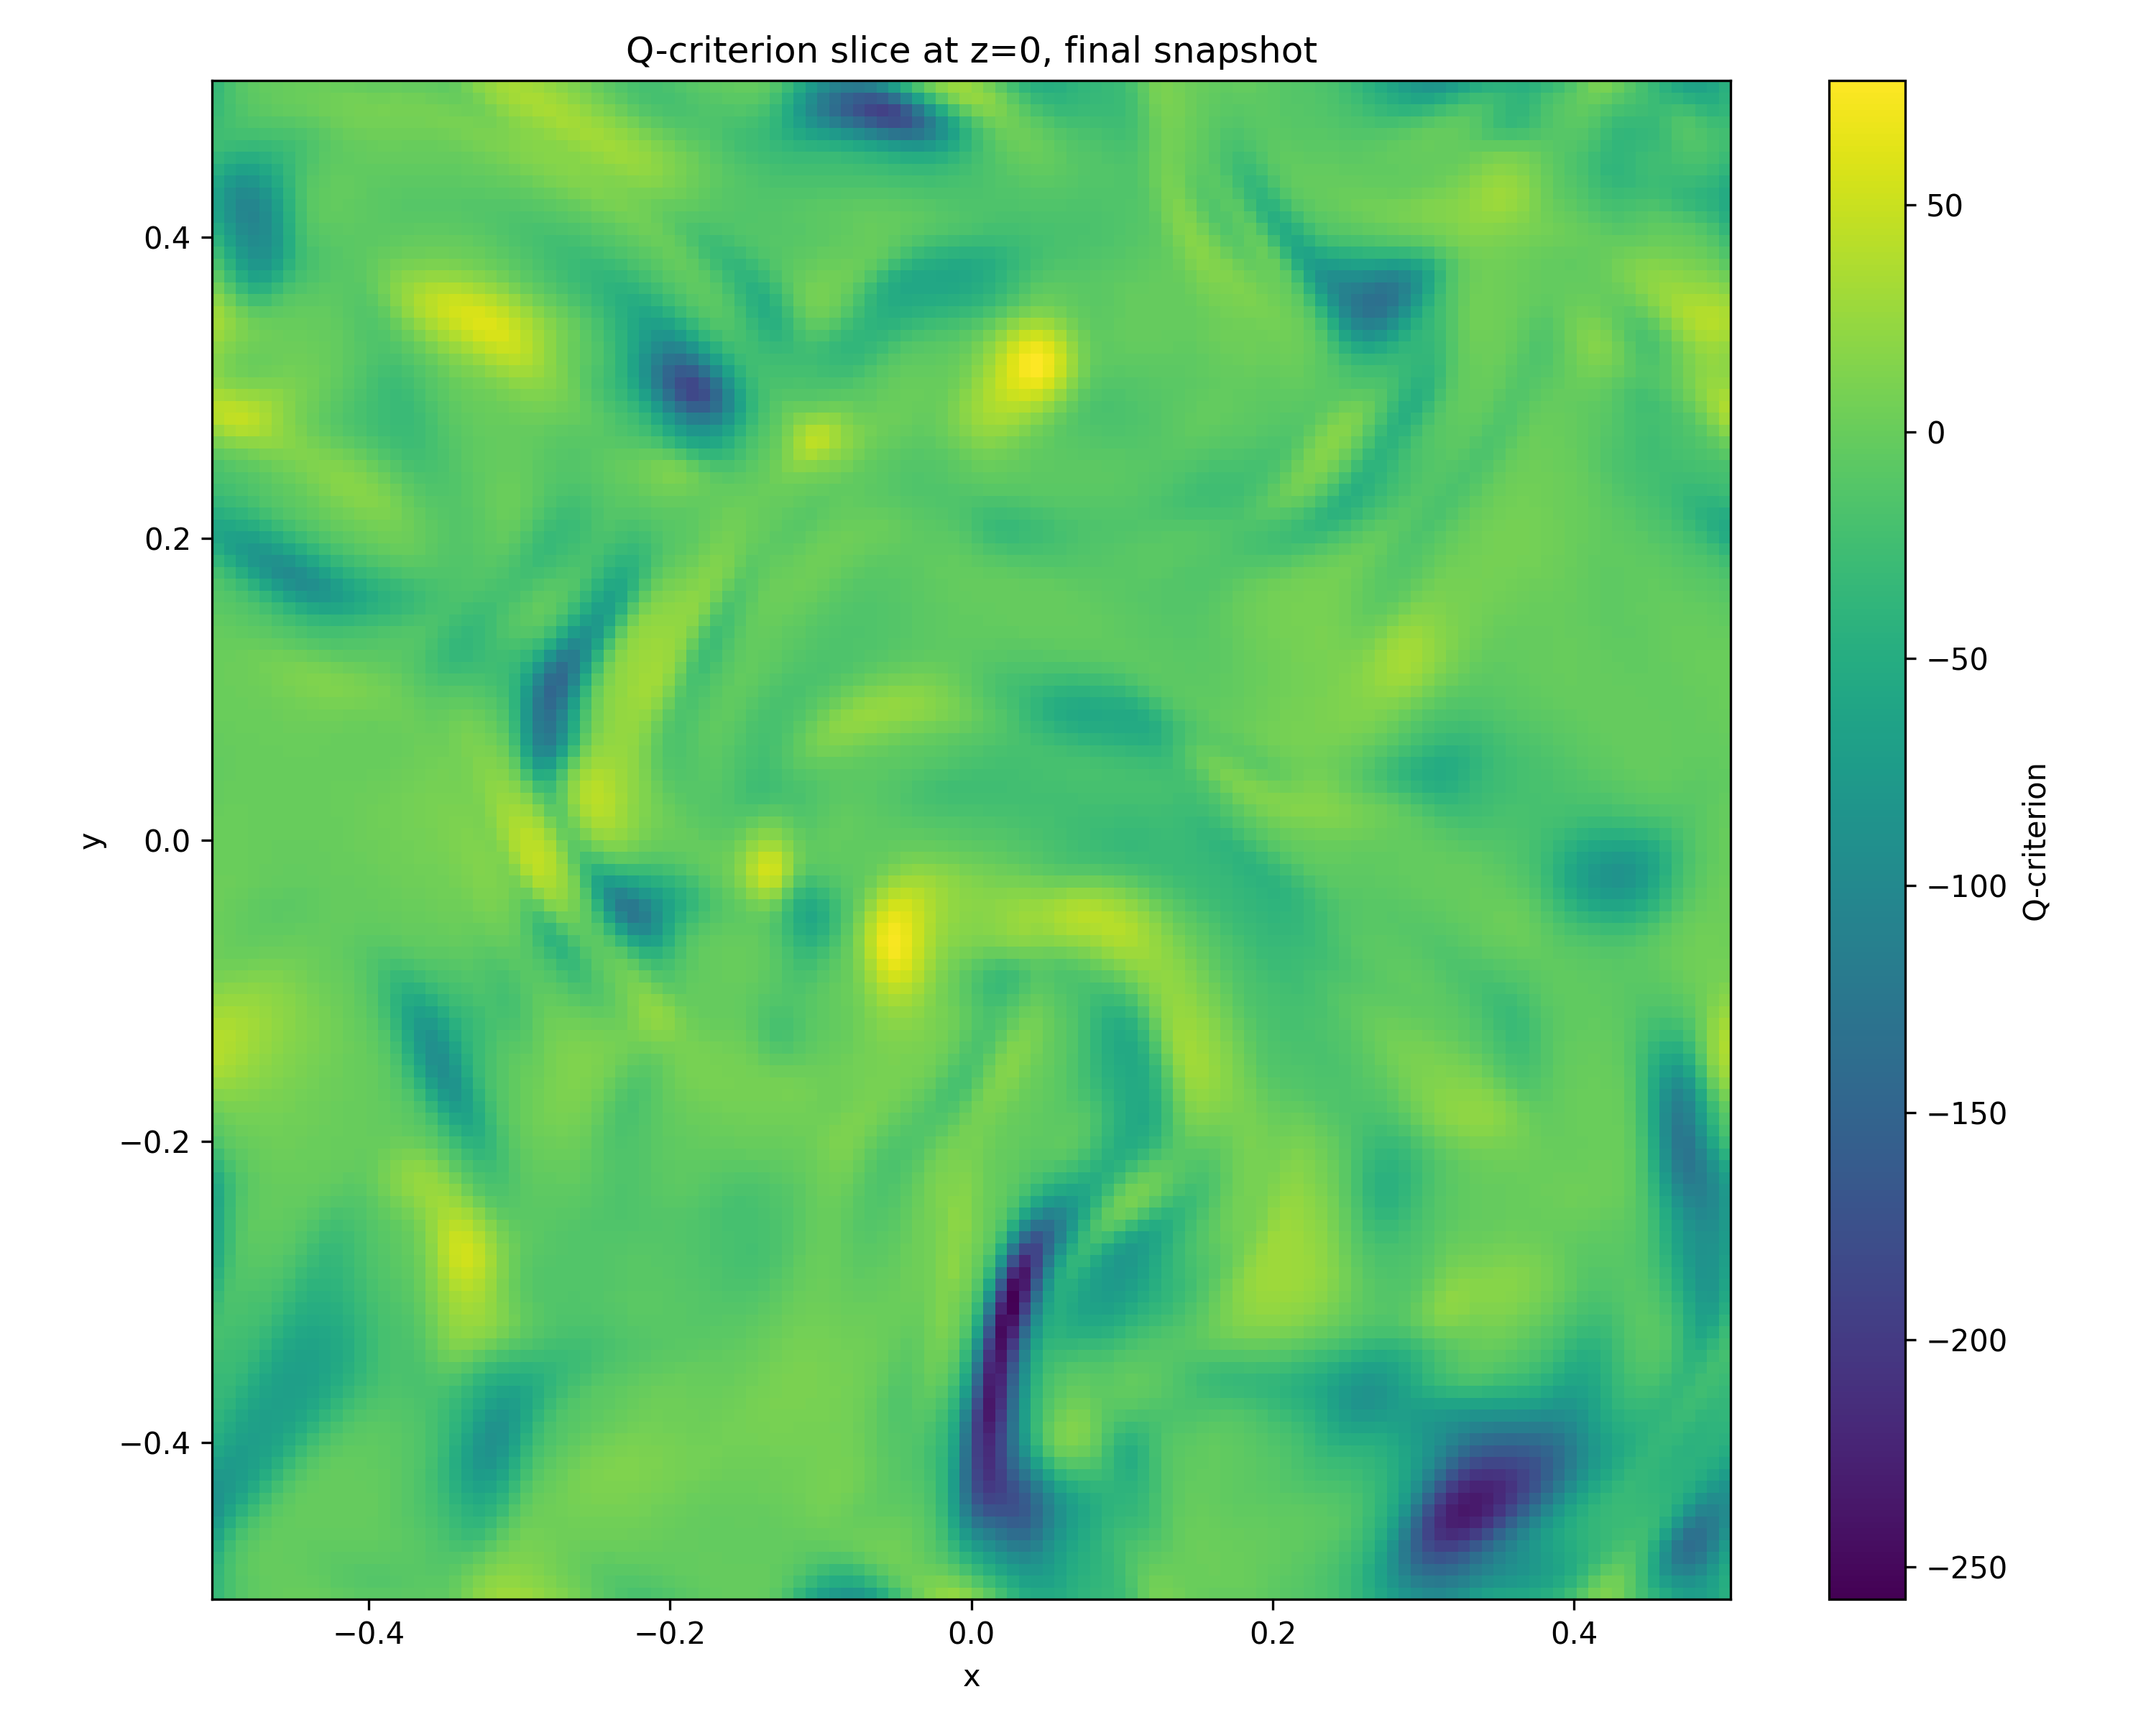
\includegraphics[width=0.5\textwidth]{../input_files/plots/step_2_Q_criterion_slice_1_1778068241.png}
    \caption{A two-dimensional slice of the Q-criterion field at z=0 from the final simulation snapshot, visualizing the instantaneous structure of the turbulent flow. Regions of positive Q-criterion (yellow) identify vortex cores where rotation dominates strain, acting as temporary trapping sites for passive tracers. Conversely, regions of large negative Q-criterion (purple) are dominated by strain. The complex field of these transient vortical and high-strain structures governs the overall transport and diffusion dynamics.}
    \label{fig:image6}
\end{figure}

\subsection{Temporal evolution of tracer dispersion}

The primary measure of transport, the ensemble-averaged Mean-Square Displacement (MSD), is presented in Figure \ref{fig:image1}. The evolution of the MSD reveals four distinct transport regimes, characterized by the local logarithmic slope $\alpha(t) = d(\log \text{MSD}) / d(\log t)$. At very early times ($t < 0.3$), transport is ballistic ($\alpha \approx 2$), as tracers move with their initial velocity. This is followed by a superdiffusive crossover regime ($0.3 < t < 1.5$) where $\alpha$ gradually decreases from approximately 1.7 to 1. The system then enters a diffusive regime ($\alpha \approx 1$) for $1.5 < t < 4$. The physical diffusion coefficient, estimated from the integral of the velocity autocorrelation function before the onset of saturation, is $D \approx 0.010$.

At late times ($t > 4$), the MSD begins to flatten, and $\alpha(t)$ drops significantly below unity. This behavior is not indicative of physical subdiffusion but is an artifact of geometric saturation. As tracers explore the entire periodic domain of side length $L=1$, their maximum possible squared displacement is limited, approaching the theoretical saturation value of $L^2/6 \approx 0.167$. By the end of the simulation, 82.9\% of tracers have crossed a periodic boundary, confirming that late-time statistics are dominated by these finite-domain effects.

Figure \ref{fig:image1} also shows a conditional MSD analysis, comparing tracers that spend the most time in vortex cores (Trapped cohort) with those that spend the least (Free cohort). The MSD of the Trapped cohort is systematically lower at all time lags, quantifying the retarding effect of vortex trapping on macroscopic transport.

\begin{figure}[h!]
    \centering
    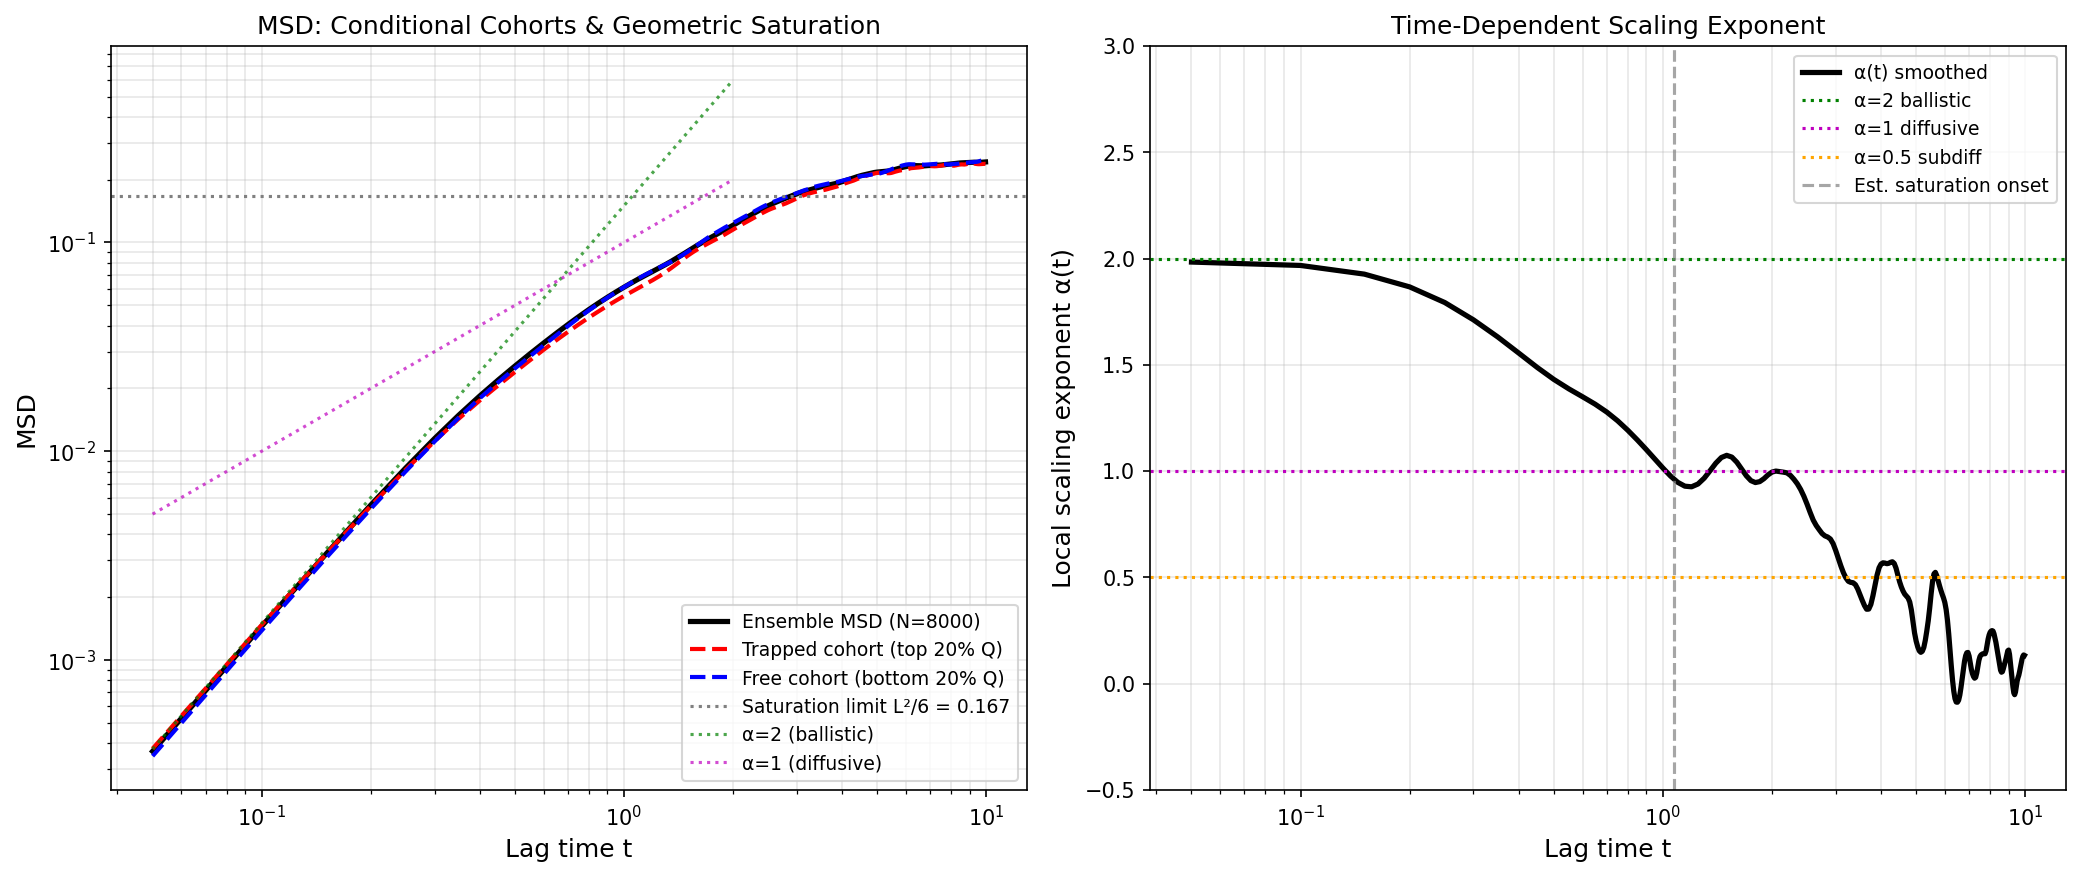
\includegraphics[width=0.5\textwidth]{../input_files/plots/step_8_MSD_conditional_1778069999.png}
    \caption{Mean-Square Displacement (MSD) and its local scaling exponent $\alpha(t)$. (Left) The ensemble-averaged MSD for 8,000 tracers transitions from ballistic ($\alpha \approx 2$) to nearly diffusive ($\alpha \approx 1$) transport before reaching the geometric saturation limit $L^2/6$. The conditional analysis shows that tracers spending more time in vortices (Trapped cohort, top 20\% Q-criterion residence) have a systematically lower MSD than those that are less trapped (Free cohort), quantifying the transport reduction due to vortex trapping. (Right) The scaling exponent $\alpha(t)$ highlights these regimes and shows that the late-time drop below unity is an artifact of this geometric saturation, not physical subdiffusion.}
    \label{fig:image1}
\end{figure}

\subsection{Transverse-dominant anisotropic dispersion}

To investigate the directional properties of the transport, we decomposed the MSD into components parallel ($\text{MSD}_{\parallel}$) and perpendicular ($\text{MSD}_{\perp}$) to the instantaneous local large-scale velocity field. The resulting anisotropy ratio, $\lambda(t) = \text{MSD}_{\parallel}(t) / \text{MSD}_{\perp}(t)$, is shown in Figure \ref{fig:image3}.

During the initial ballistic phase ($t < 0.5$), the anisotropy ratio peaks at $\lambda \approx 2.96$, indicating that initial displacements are preferentially aligned with the large-scale flow. However, as tracers begin to decorrelate from their initial velocity, the ratio rapidly drops below unity. For $t > 0.5$, the anisotropy stabilizes at a mean value of $\lambda \approx 0.52 \pm 0.045$. This result, $\lambda < 1$, reveals a persistent and significant anisotropy where dispersion perpendicular to the local large-scale velocity systematically exceeds parallel dispersion. This transverse-dominant transport is a direct kinematic signature of the solenoidal forcing, where large-scale rotational motions are more efficient at sweeping tracers in the transverse plane than advection is at carrying them along the flow direction.

\begin{figure}[h!]
    \centering
    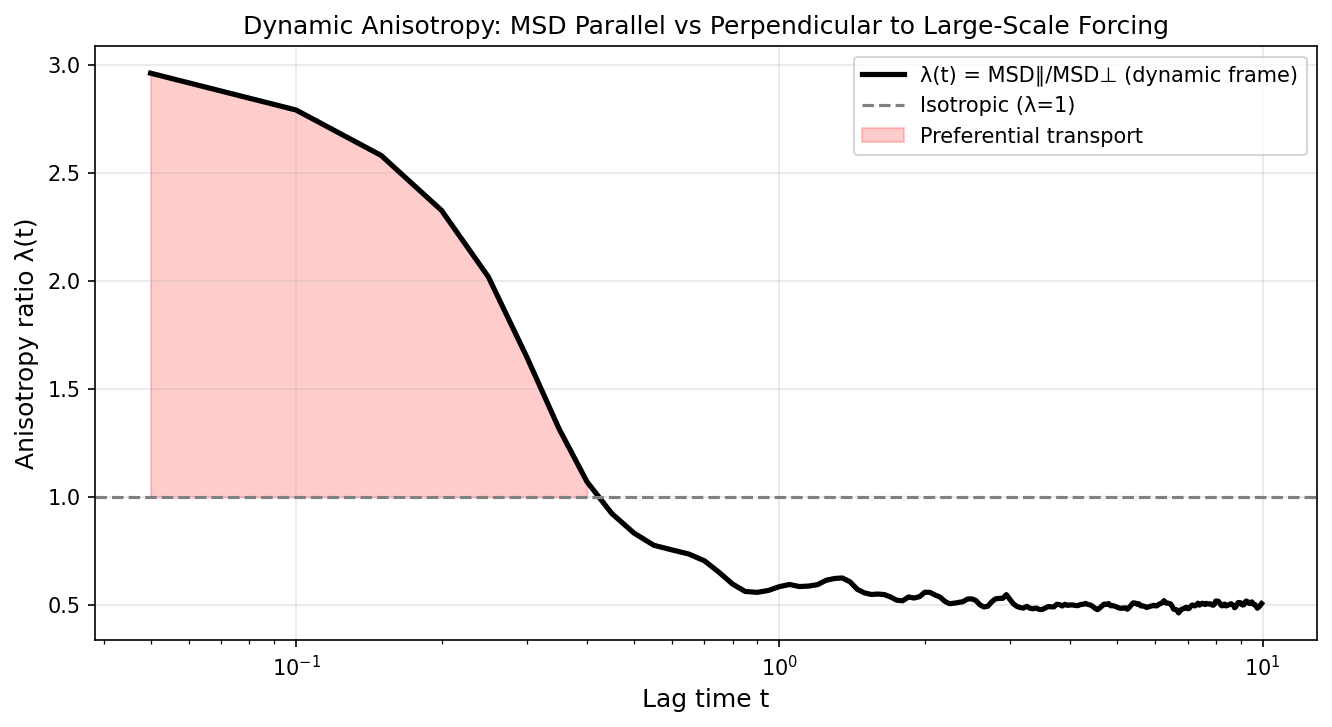
\includegraphics[width=0.5\textwidth]{../input_files/plots/step_8_anisotropy_1778069999.png}
    \caption{Dynamic anisotropy ratio $\lambda(t) = \text{MSD}_{\parallel} / \text{MSD}_{\perp}$, where the Mean-Square Displacement (MSD) is decomposed relative to the instantaneous large-scale velocity. After an initial ballistic phase where transport is preferentially parallel to the flow ($\lambda > 1$ for $t < 0.5$), the ratio drops and stabilizes below unity to a mean of $\lambda \approx 0.52$. This reversal demonstrates that perpendicular dispersion exceeds parallel dispersion at later times, a signature of solenoidal forcing where vortical motions spread tracers more effectively in the transverse direction than advection along the main flow.}
    \label{fig:image3}
\end{figure}

\subsection{Transient nature of vortex trapping}

The observation of a superdiffusive crossover regime motivates an investigation into its physical origin, particularly the role of vortex trapping. To quantify the duration of trapping events, we computed the Lagrangian autocorrelation function of the Q-criterion signal along tracer trajectories, shown in Figure \ref{fig:image2}. The function exhibits a rapid decay, crossing the $1/e$ threshold at a characteristic timescale of $\tau_Q \approx 0.200$.

Comparing this trapping timescale to the large-eddy turnover time, $T_e = L/v_{\text{rms}} \approx 1/0.38 \approx 2.6$, we find that $\tau_Q / T_e \approx 0.077$. This demonstrates that tracers remain trapped within a coherent vortex for only about 7-8\% of a large-eddy turnover time. These trapping events are highly transient, likely terminated by three-dimensional vortex instabilities such as stretching and bending. The short residence times are insufficient to generate the long-term memory required for sustained anomalous transport phenomena, such as Lévy flights, explaining the eventual return to a diffusive regime.

\begin{figure}[h!]
    \centering
    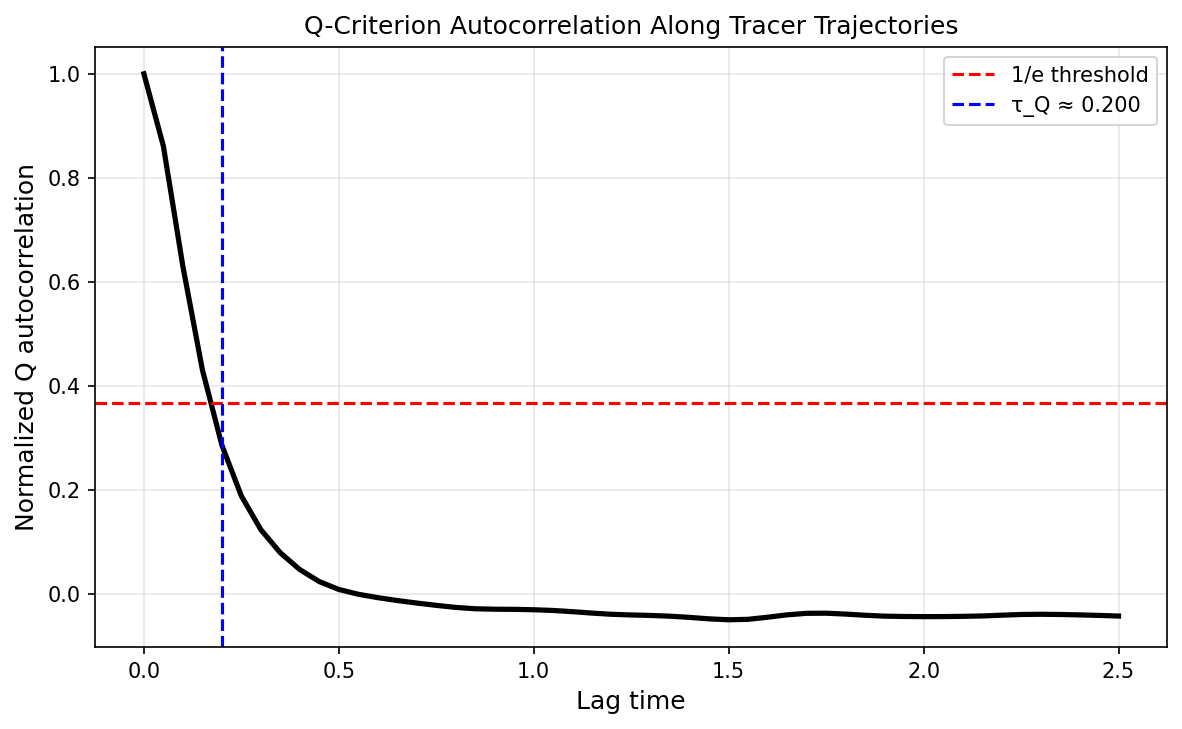
\includegraphics[width=0.5\textwidth]{../input_files/plots/step_8_Q_autocorr_1778069999.png}
    \caption{Autocorrelation of the Q-criterion along Lagrangian tracer trajectories. The correlation decays rapidly, defining a vortex trapping timescale, $\tau_{Q} \approx 0.200$, where the function drops to 1/e of its initial value. This short timescale, corresponding to approximately 7-8\% of a large-eddy turnover time, indicates that trapping events are too transient to generate the heavy-tailed waiting-time distributions characteristic of Lévy flights.}
    \label{fig:image2}
\end{figure}

\subsection{Statistical properties of tracer displacements}

The statistical nature of the transport process is further elucidated by the Probability Density Functions (PDFs) of tracer displacements, shown in Figure \ref{fig:image4}. At early times ($t=0.5, 1.0$), the distributions exhibit mild non-Gaussian features, consistent with the presence of velocity correlations during the superdiffusive crossover. By an intermediate time of $t=2.0$, the displacement PDF is statistically indistinguishable from a Gaussian distribution, as confirmed by a Kolmogorov-Smirnov test ($p=0.53$).

Crucially, at late times ($t=5.0, 9.0$), the PDFs deviate significantly from Gaussian, but not by developing heavy tails. Instead, they become platykurtic (light-tailed and flat-topped), with an excess kurtosis approaching -1.2. This platykurtic shape is a direct consequence of the geometric saturation discussed previously; as tracers are confined within the periodic domain, their displacement distribution becomes more uniform and bounded. A Hill estimator applied to the distribution tails yields a power-law exponent of $\alpha_L \approx -7.1$, confirming the absence of the heavy tails ($0 < \alpha_L \leq 2$) that characterize Lévy flights.

\begin{figure}[h!]
    \centering
    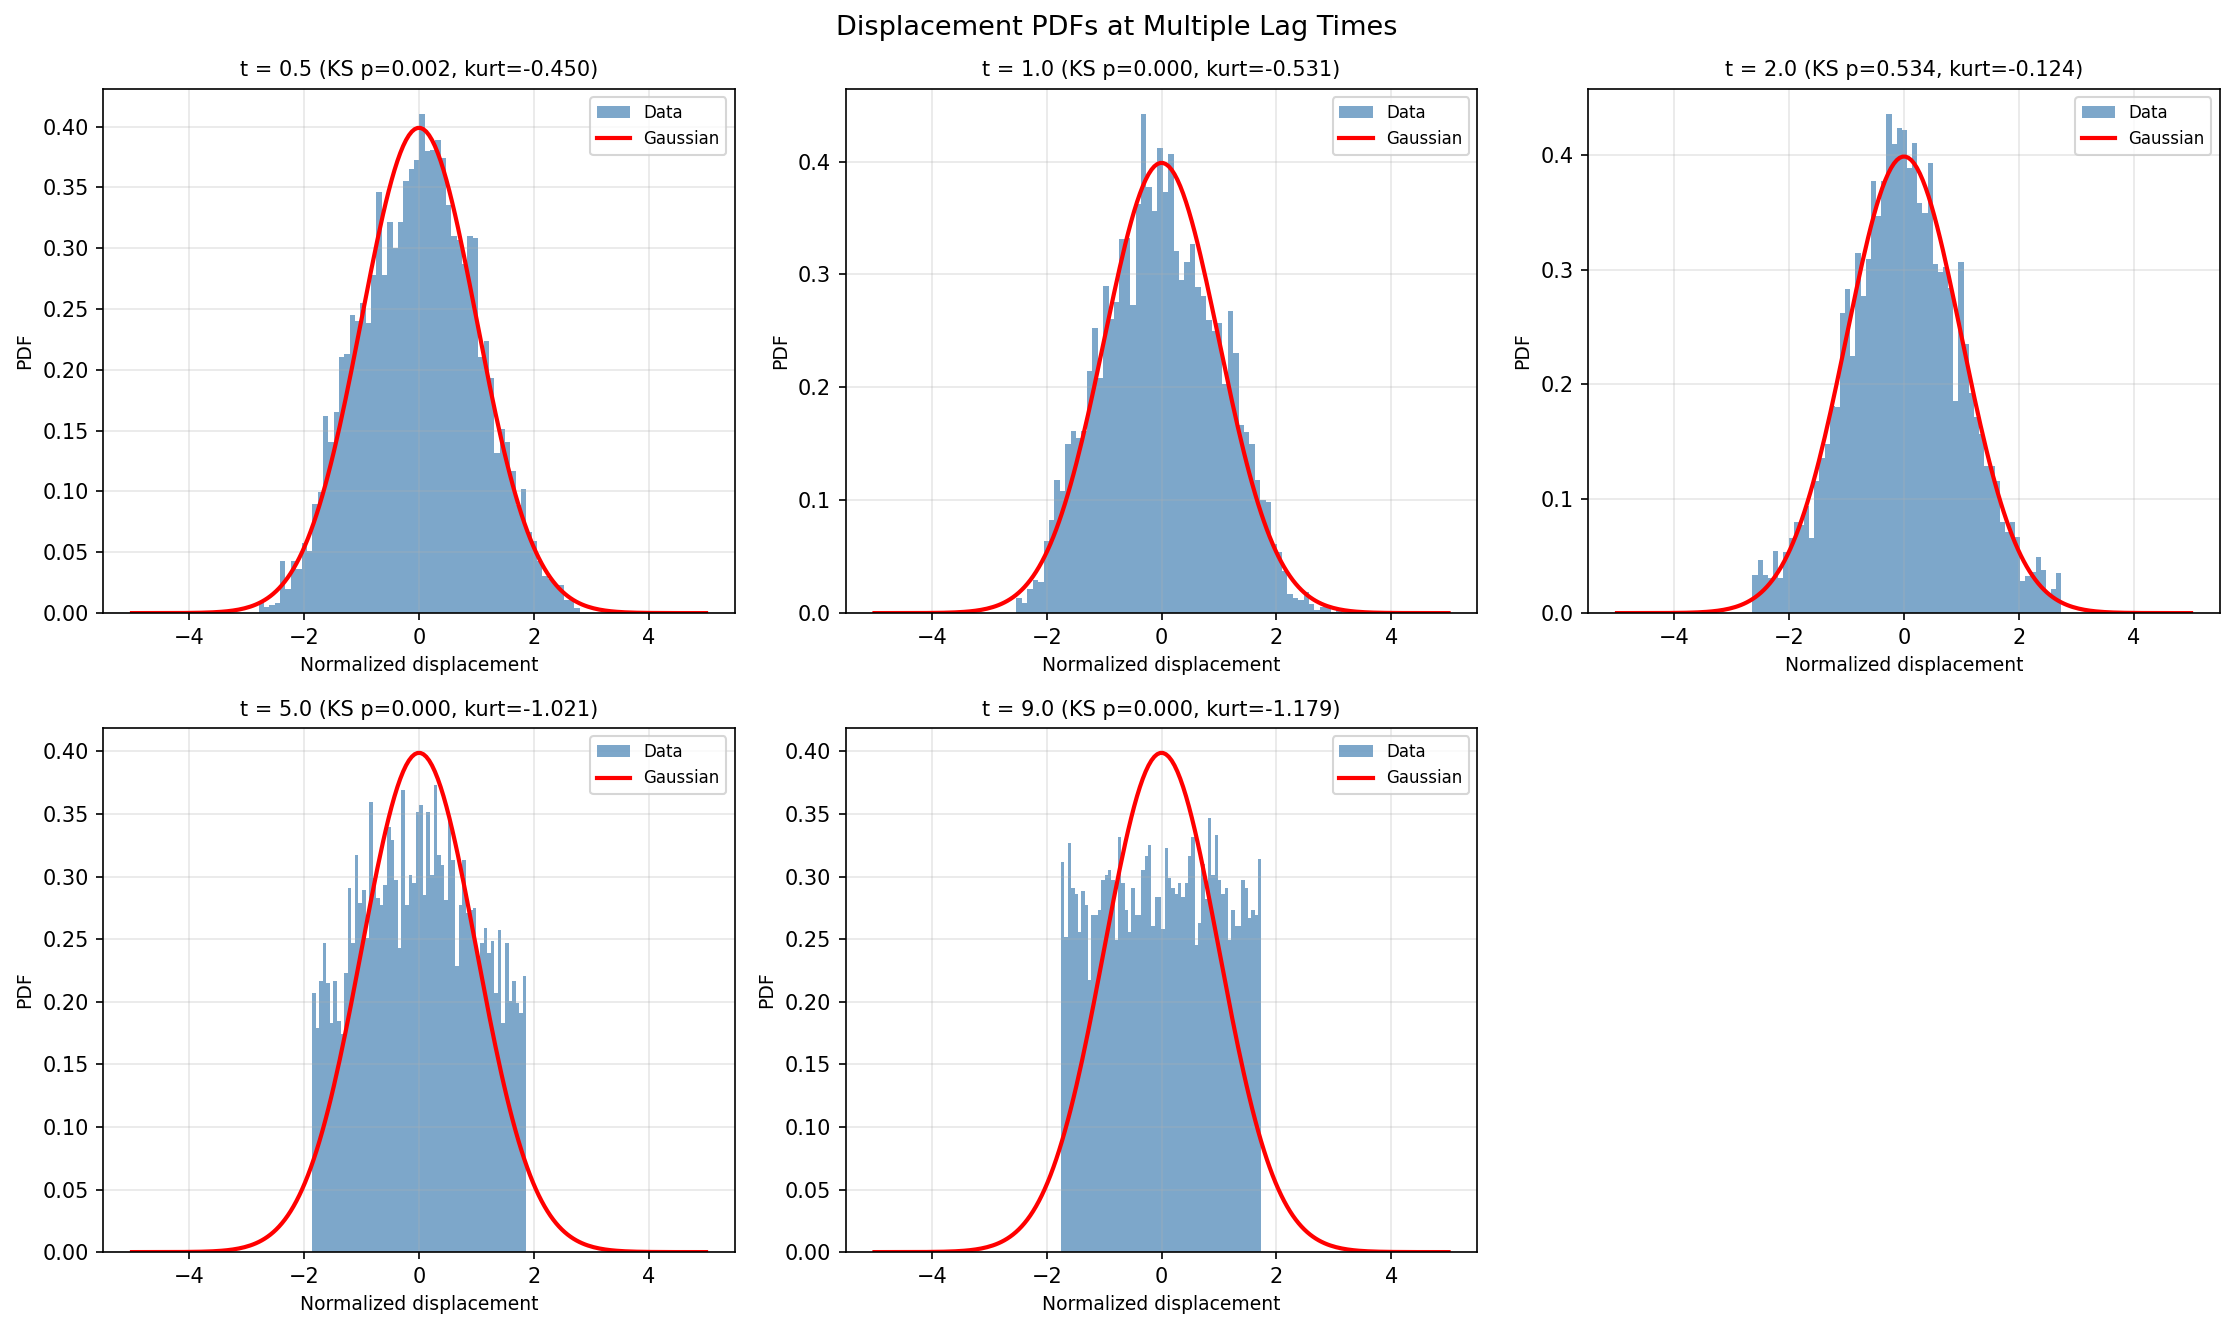
\includegraphics[width=0.5\textwidth]{../input_files/plots/step_8_displacement_PDFs_1778069999.png}
    \caption{Probability Density Functions (PDFs) of normalized tracer displacements at multiple lag times, compared with a Gaussian distribution (red line). The distributions transition from mildly non-Gaussian at early times (t = 0.5, 1.0) to being indistinguishable from Gaussian at an intermediate time (t = 2.0, KS p-value = 0.53). At late times (t = 5.0, 9.0), the PDFs become significantly platykurtic (flat-topped) with large negative excess kurtosis, a signature of geometric saturation in the finite periodic domain rather than the heavy tails associated with anomalous transport.}
    \label{fig:image4}
\end{figure}

\subsection{Role of chaotic dynamics}

Finally, we explored the connection between chaotic stretching and tracer dynamics using the Finite-Time Lyapunov Exponent (FTLE), a measure of trajectory separation. The long-time FTLE, calculated over the full trajectory, proves to be a weak indicator of the underlying dynamics in the periodic domain. The FTLE distributions are narrow and centered near zero, reflecting the bounded relative separation of tracers. As shown in Figure \ref{fig:image0}, the FTLE distributions for the Trapped and Free tracer cohorts are nearly identical, with statistically indistinguishable mean values ($-0.008 \pm 0.013$ for Trapped vs. $-0.007 \pm 0.013$ for Free).

This lack of correlation is reinforced in Figure \ref{fig:image5} (left panel), which shows no relationship between a tracer's long-time FTLE and its residence fraction in vortices (Pearson r = 0.002). We also investigated whether tracers are ejected from vortices through regions of high strain by measuring the FTLE at the instant of vortex exit (Figure \ref{fig:image5}, right panel). The mean FTLE at exit points ($-0.010$) is only marginally lower than the ensemble average. This provides modest support for the hypothesis that ejection is strain-driven, but the signal is weak in the long-time FTLE metric. A shorter-timescale FTLE would be necessary to test this causal link more sharply.

\begin{figure}[h!]
    \centering
    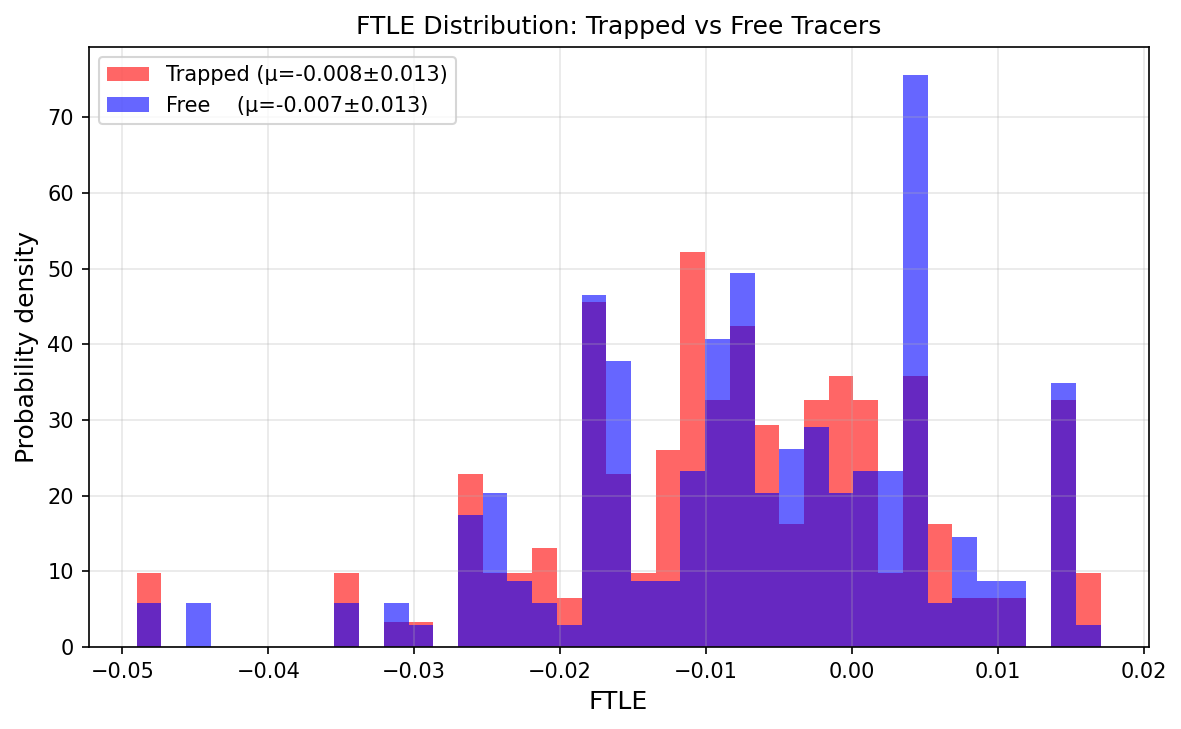
\includegraphics[width=0.5\textwidth]{../input_files/plots/step_8_FTLE_cohorts_1778069999.png}
    \caption{Probability density distribution of the Finite-Time Lyapunov Exponent (FTLE) for tracers classified as Trapped (red) or Free (blue) based on their residence time in high-vorticity regions. The distributions for both cohorts are nearly identical and centered close to zero, with mean FTLE values of -0.008 ± 0.013 for the Trapped cohort and -0.007 ± 0.013 for the Free cohort. This indicates that the long-time FTLE, measured over the full trajectory within the periodic domain, does not effectively distinguish between the dynamics of tracers trapped in vortices and those moving freely.}
    \label{fig:image0}
\end{figure}

\begin{figure}[h!]
    \centering
    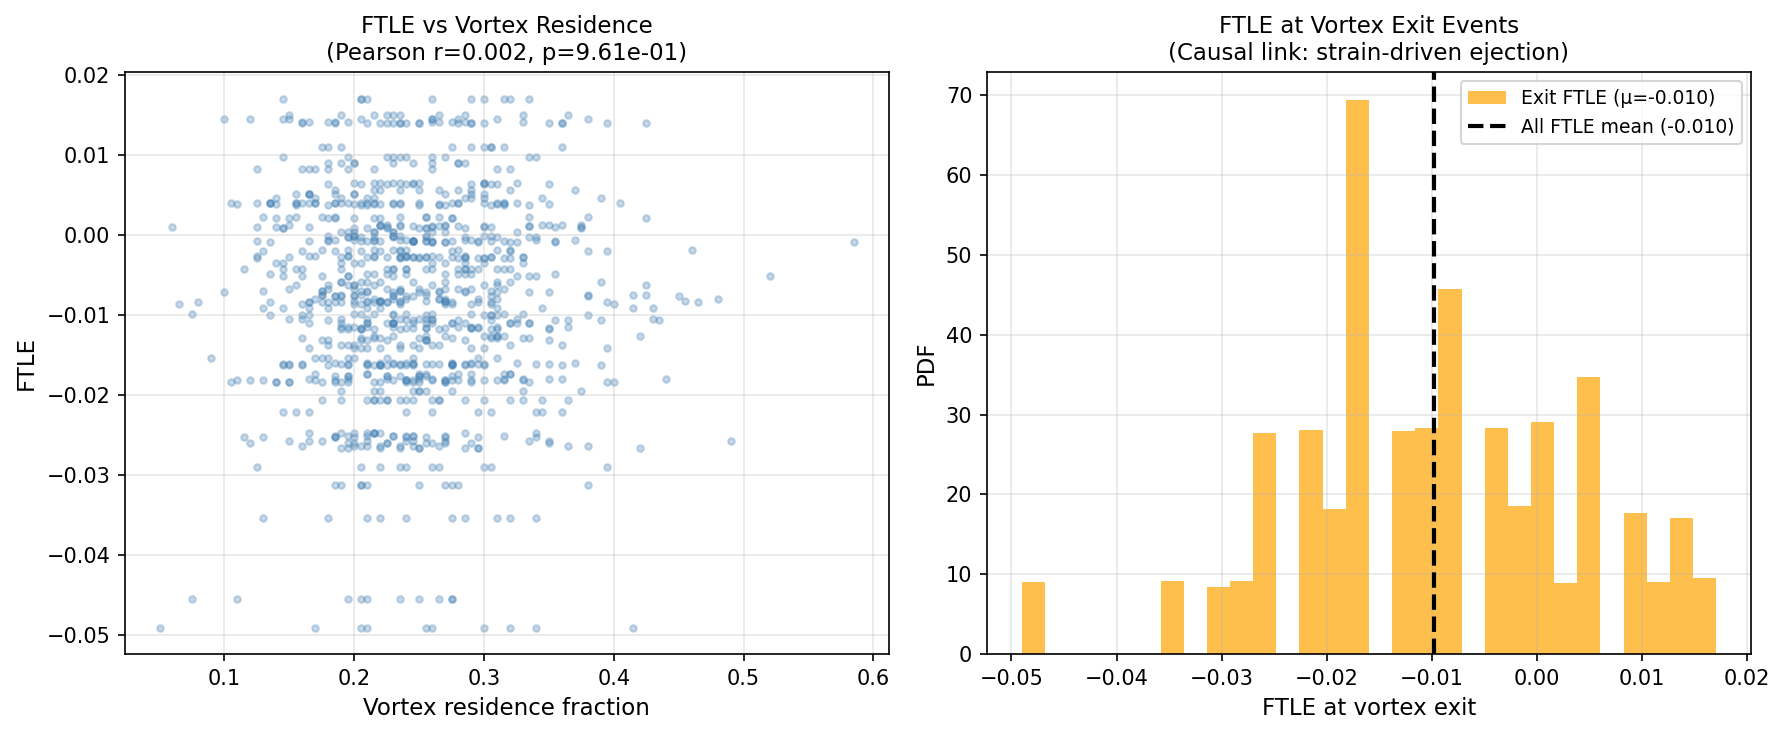
\includegraphics[width=0.5\textwidth]{../input_files/plots/step_8_exit_FTLE_1778069999.png}
    \caption{Analysis of chaotic dynamics and vortex ejection. (Left) The long-time Finite-Time Lyapunov Exponent (FTLE) shows no correlation with the vortex residence fraction of tracers (Pearson r = 0.002), indicating that long-term chaoticity is independent of trapping duration. (Right) The distribution of FTLE values at the instant of vortex exit has a mean ($\mu$ = -0.010) nearly identical to the ensemble average, suggesting that ejection events are not strongly associated with regions of anomalously high chaotic stretching as measured by this long-time metric.}
    \label{fig:image5}
\end{figure}

\section{Conclusions}
\label{sec:conclusions}
In this study, we investigated the transport of passive Lagrangian tracers in a direct numerical simulation of three-dimensional, subsonic turbulence driven by large-scale solenoidal forcing. The primary goal was to understand how the rotational nature of the energy injection and the resulting coherent vortex structures influence the statistical properties of particle dispersion, specifically its anisotropy and potential for anomalous transport. To this end, we analyzed the trajectories of thousands of tracers, focusing on the Mean-Square Displacement, its decomposition relative to the large-scale flow, the duration of vortex trapping events, and the evolution of displacement probability distributions.

Our analysis revealed two principal findings. First, we identified a persistent and strong anisotropy in the dispersion process. After an initial ballistic phase where particle motion is aligned with the large-scale velocity, the transport becomes dominated by dispersion perpendicular to the local flow direction. The anisotropy ratio stabilizes at a value of approximately 0.52, indicating that transverse transport is nearly twice as effective as parallel transport. This transverse-dominant dispersion is a direct kinematic signature of the solenoidal forcing, where large-scale rotational motions sweep particles more efficiently across the flow than advection carries them along it.

Second, we examined the hypothesis that vortex trapping is a primary driver of anomalous transport. While we confirmed that tracers are transiently captured by coherent vortex structures, we found that these trapping events are remarkably brief. The characteristic residence time within a vortex is only about 7\% of a large-eddy turnover time. These short trapping durations, likely limited by three-dimensional vortex instabilities, are insufficient to generate the long-term memory required for sustained superdiffusion or Lévy-flight statistics. Consequently, the probability distributions of tracer displacements do not develop heavy tails; they are nearly Gaussian at intermediate times and become platykurtic (light-tailed) at late times due to the geometric constraints of the finite periodic domain.

From these results, we conclude that in three-dimensional solenoidal turbulence, the forward energy cascade and inherent vortex dynamics effectively suppress long-range temporal correlations in tracer trajectories. Although the solenoidal forcing imposes a strong and persistent anisotropy on the transport, it does not lead to a breakdown of classical diffusion in the long-time limit. The system robustly returns to a diffusive regime, highlighting that the presence of coherent structures alone is not a sufficient condition for generating anomalous transport.


\bibliography{bibliography}{}
\bibliographystyle{unsrt}

\end{document}
